\subsection{パターン認識}
パターン認識とは予め与えられた大量のデータ(学習データ; 一般にはクラス既知)利用して,クラス未知のデータ(テストデータ)が, どのクラスに属するか推定する問題である.\\
パターン認識の方法として
\begin{enumerate}
\item 与えられた学習データをベクトル表現に置き換える($x_{1},\ x_{2},\ x_{3},\ x_{4}$)\\
\item 特徴ベクトル空間上での分布を調べる
\begin{center}
  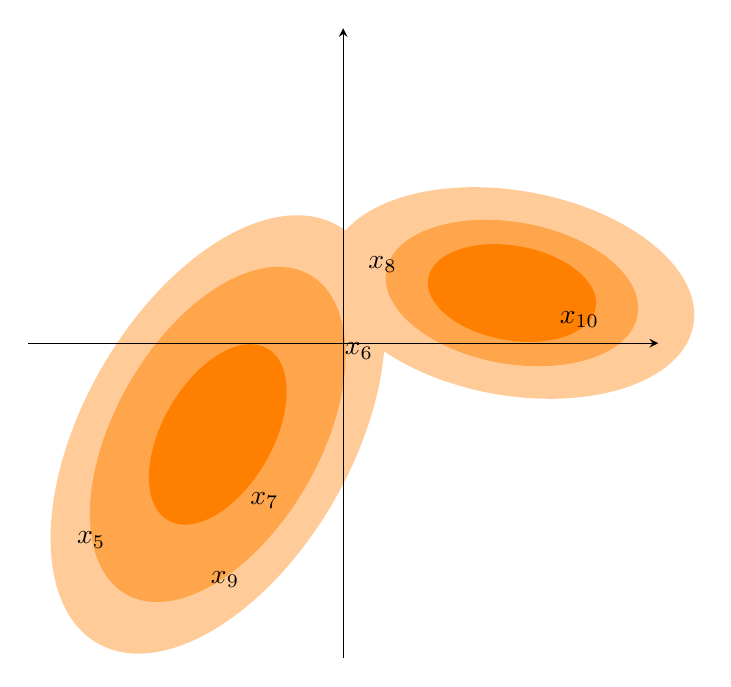
\begin{tikzpicture}[>=stealth]
    \fill[fill=orange!40,rotate=60] (-1.8,0.8) circle[xscale=1.8,radius=1.7];
    \fill[fill=orange!40,rotate=-10] (2,1) circle[xscale=1.8,radius=1.3];
    \fill[fill=orange!70,rotate=60] (-1.8,0.8) circle[xscale=1.8,radius=1.3];
    \fill[fill=orange,rotate=60] (-1.8,0.8) circle[xscale=1.8,radius=0.7];
    \fill[fill=orange!70,rotate=-10] (2,1) circle[xscale=1.8,radius=0.9];
    \fill[fill=orange,rotate=-10] (2,1) circle[xscale=1.8,radius=0.6];
    \draw[->](-4,0)--(4,0);
    \draw[->](0,-4)--(0,4);
    \node at(0.2,-0.1) {$x_{6}$};
    \node at(3,0.3) {$x_{10}$};
    \node at(0.5,1) {$x_{8}$};
    \node at(-1,-2) {$x_{7}$};
    \node at(-1.5,-3) {$x_{9}$};
    \node at(-3.2,-2.5) {$x_{5}$};
  \end{tikzpicture}
\end{center}
\item 分布を元にクラスの境界を定める.
\begin{center}
    \begin{tikzpicture}[>=stealth,scale=1.2]
        \fill[fill=orange!40,rotate=60] (-3,1.7) circle[xscale=1.9,radius=1.3];
        \fill[fill=orange!40,rotate=-5] (-0.7,0.3) circle[xscale=1.8,radius=1];
        \fill[fill=orange!70,rotate=60] (-3,1.7) circle[xscale=1.9,radius=1.1];
        \fill[fill=orange!70,rotate=-5] (-0.7,0.3) circle[xscale=1.8,radius=0.7];
        \fill[fill=orange,rotate=60] (-3,1.7) circle[xscale=1.9,radius=0.7];
        \fill[fill=orange,rotate=-5] (-0.7,0.3) circle[xscale=1.8,radius=0.3];

        \fill[fill=orange!40,rotate=93] (0,-2.9) circle[xscale=2.8,radius=0.9];
        \fill[fill=orange!40,rotate=5] (1.3,-2.2) circle[xscale=2,radius=0.9];
        \fill[fill=orange!70,rotate=93] (0,-2.9) circle[xscale=2.5,radius=0.5];
        \fill[fill=orange!70,rotate=5] (1.3,-2.2) circle[xscale=2,radius=0.6];
        \fill[fill=orange,rotate=93] (0,-2.9) circle[xscale=2.5,radius=0.3];
        \fill[fill=orange,rotate=5] (1.3,-2.2) circle[xscale=2,radius=0.3];
        \draw [draw=blue,very thick](-1.5,2.5) to [out=340,in=90] (1.5,0) to [out=270,in=10] (-0.5,-1.2) to[out=190,in=85] (-1.5,-3) to [out=265,in=110] (-1.4,-4);
        \draw[->] (-4,0)--(4,0);
        \draw[->] (0,-4)--(0,4);
        \fill[fill=red] (0.2,0.3) circle[radius=0.1];
        \node at(-0.1,0.4) {$\mbox{\boldmath $x$}$};
        \node at(-3.7,1) {Aの分布};
        \node at(4,1) {Bの分布};
  \end{tikzpicture}
\end{center}
\item テストデータのベクトル($\mbox{\boldmath $x$}$)が境界のどちら側にあるかを調べることで, テストデータ($x$)のクラスを定める.
\end{enumerate}
\subsection{線形識別}
\begin{center}
    \begin{tikzpicture}[>=stealth,scale=1.2]
        \fill[fill=orange!40,rotate=60] (-3,1.7) circle[xscale=1.9,radius=1.3];
        \fill[fill=orange!40,rotate=-5] (-0.7,0.3) circle[xscale=1.8,radius=1];
        \fill[fill=orange!70,rotate=60] (-3,1.7) circle[xscale=1.9,radius=1.1];
        \fill[fill=orange!70,rotate=-5] (-0.7,0.3) circle[xscale=1.8,radius=0.7];
        \fill[fill=orange,rotate=60] (-3,1.7) circle[xscale=1.9,radius=0.7];
        \fill[fill=orange,rotate=-5] (-0.7,0.3) circle[xscale=1.8,radius=0.3];

        \fill[fill=orange!40,rotate=93] (0,-2.9) circle[xscale=2.8,radius=0.9];
        \fill[fill=orange!40,rotate=5] (1.3,-2.2) circle[xscale=2,radius=0.9];
        \fill[fill=orange!70,rotate=93] (0,-2.9) circle[xscale=2.5,radius=0.5];
        \fill[fill=orange!70,rotate=5] (1.3,-2.2) circle[xscale=2,radius=0.6];
        \fill[fill=orange,rotate=93] (0,-2.9) circle[xscale=2.5,radius=0.3];
        \fill[fill=orange,rotate=5] (1.3,-2.2) circle[xscale=2,radius=0.3];
        \draw[->] (-4,0)--(4,0);
        \draw[->] (0,-4)--(0,4);
        \fill[fill=red] (0.2,0.3) circle[radius=0.1];
        \node at(-0.1,0.4) {$\mbox{\boldmath $x$}$};
        \node at(-3.7,1) {Aの分布};
        \node at(4,1) {Bの分布};
        \draw[very thick,draw=blue] (-1.3,3.5)--(1,-3.5);
        \filldraw[draw=blue,fill=cyan!30,opacity=0.4] (0.3,0.3) circle[radius=0.5];
        \filldraw[draw=blue,fill=cyan!30,opacity=0.4] (-0.2,-2.3) circle[radius=0.73];
  \end{tikzpicture}
\end{center}
線形識別においては図の水色で囲んでいるところが誤認識となる領域となる. 識別平面の設定によって, 誤認識となる領域が変わる.
以下のように識別平面の設定によると先の場合より領域が小さくなる.
\begin{center}
  \begin{tikzpicture}[>=stealth,scale=1.2]
    \fill[fill=orange!40,rotate=60] (-3,1.7) circle[xscale=1.9,radius=1.3];
    \fill[fill=orange!40,rotate=-5] (-0.7,0.3) circle[xscale=1.8,radius=1];
    \fill[fill=orange!70,rotate=60] (-3,1.7) circle[xscale=1.9,radius=1.1];
    \fill[fill=orange!70,rotate=-5] (-0.7,0.3) circle[xscale=1.8,radius=0.7];
    \fill[fill=orange,rotate=60] (-3,1.7) circle[xscale=1.9,radius=0.7];
    \fill[fill=orange,rotate=-5] (-0.7,0.3) circle[xscale=1.8,radius=0.3];

    \fill[fill=orange!40,rotate=93] (0,-2.9) circle[xscale=2.8,radius=0.9];
    \fill[fill=orange!40,rotate=5] (1.3,-2.2) circle[xscale=2,radius=0.9];
    \fill[fill=orange!70,rotate=93] (0,-2.9) circle[xscale=2.5,radius=0.5];
    \fill[fill=orange!70,rotate=5] (1.3,-2.2) circle[xscale=2,radius=0.6];
    \fill[fill=orange,rotate=93] (0,-2.9) circle[xscale=2.5,radius=0.3];
    \fill[fill=orange,rotate=5] (1.3,-2.2) circle[xscale=2,radius=0.3];
    \draw[->] (-4,0)--(4,0);
    \draw[->] (0,-4)--(0,4);
    \fill[fill=red] (0.2,0.3) circle[radius=0.1];
    \node at(-0.1,0.4) {$\mbox{\boldmath $x$}$};
    \node at(-3.7,1) {Aの分布};
    \node at(4,1) {Bの分布};
    \draw[very thick,draw=blue] (2.3,3.5)--(-0.5,-3.5);
    \filldraw[draw=blue,fill=cyan!30,opacity=0.4] (1,0.1) circle[radius=0.4];
    \filldraw[draw=blue,fill=cyan!30,opacity=0.4] (-0.2,-2.1) circle[radius=0.4];
  \end{tikzpicture}
\end{center}
線形識別においてクラスAの分布を$f(x)=0$,\ クラスBの分布を$f(x)=1$とする.ここで,
\begin{eqnarray*}
  y=g(x;\Theta)
\end{eqnarray*}
とすることでロジスティック回帰分析を行う.
%%%ここからが新しいところ
\begin{center}
  \begin{tikzpicture}[>=stealth]
    \node at(-4,6) {\includegraphics[width=6cm]{senkei.png}};
    \draw[very thick,->] (-6,0)--(6,0) node[right]{$y$};
    \draw[very thick,->] (-0.5,-0.3)--(-0.5,3.5);
    %%
    \fill[fill=blue] (-4,4.5) circle[radius=0.1];
    \fill[fill=blue] (-2,5) circle[radius=0.1];
    \fill[fill=red] (-6.8,4.5) circle[radius=0.1];
    \fill[fill=red] (-5,5.2) circle[radius=0.1];
    %%
    \draw[xscale=1.5,domain=0:6,thick,draw=green] plot(\x-3,{3/(1+exp(-3*\x+8))});
    \draw[draw=gray!40](-6,3)--(6,3);
    \fill[fill=red] (-5,0) circle[radius=0.1];
    \fill[fill=red] (-2.5,0) circle[radius=0.1];
    \fill[fill=blue] (1.5,3) circle[radius=0.1];
    \fill[fill=blue] (4,3) circle[radius=0.1];
    \draw[fill=white,draw=blue] (1.5,0) circle[radius=0.1];
    \draw[fill=white,draw=blue] (4,0) circle[radius=0.1];
    \draw[<->] (1.5,0.1)--(1.5,2.9);
    \draw[<->] (4,0.1)--(4,2.9);

    \draw[->,draw=gray!80] (-6.8,4.4) to [out=270,in=180] (-5.5,3) to[out=0,in=90] (-5,0.1);
    \draw[->,draw=gray!80] (-5,5.1) to [out=270,in=180] (-4,3.2) to[out=0,in=90] (-2.5,0.1);
    \draw[->,draw=gray!80] (-3.9,4.5) to[out=0,in=120] (1.43,0.14);
    \draw[->,draw=gray!80] (-1.9,5) to[out=0,in=110] (3.94,0.14);
  \end{tikzpicture}
\end{center}
\begin{eqnarray*}
  z=f(y;\Psi) = f(g(x;\Theta);\Psi)
\end{eqnarray*}
線形識別の場合は
\begin{center}
  \begin{tikzpicture}[>=stealth,scale=1.2]
        \fill[fill=orange!40,rotate=60] (-3,1.7) circle[xscale=1.9,radius=1.3];
        \fill[fill=orange!40,rotate=-5] (-0.7,0.3) circle[xscale=1.8,radius=1];
        \fill[fill=orange!70,rotate=60] (-3,1.7) circle[xscale=1.9,radius=1.1];
        \fill[fill=orange!70,rotate=-5] (-0.7,0.3) circle[xscale=1.8,radius=0.7];
        \fill[fill=orange,rotate=60] (-3,1.7) circle[xscale=1.9,radius=0.7];
        \fill[fill=orange,rotate=-5] (-0.7,0.3) circle[xscale=1.8,radius=0.3];

        \fill[fill=orange!40,rotate=93] (0,-2.9) circle[xscale=2.8,radius=0.9];
        \fill[fill=orange!40,rotate=5] (1.3,-2.2) circle[xscale=2,radius=0.9];
        \fill[fill=orange!70,rotate=93] (0,-2.9) circle[xscale=2.5,radius=0.5];
        \fill[fill=orange!70,rotate=5] (1.3,-2.2) circle[xscale=2,radius=0.6];
        \fill[fill=orange,rotate=93] (0,-2.9) circle[xscale=2.5,radius=0.3];
        \fill[fill=orange,rotate=5] (1.3,-2.2) circle[xscale=2,radius=0.3];
        \draw[->] (-4,0)--(4,0);
        \draw[->] (0,-4)--(0,4);
        \fill[fill=red] (0.2,0.3) circle[radius=0.1];
        \fill[fill=red] (-1,0.35) circle[radius=0.1];
        \fill[fill=red] (-1.5,-0.35) circle[radius=0.1];
        \fill[fill=red] (-1.9,-0.5) circle[radius=0.1];
        \fill[fill=red] (-3,-1) circle[radius=0.1];
        \fill[fill=red] (-3.5,-2) circle[radius=0.1];
        \fill[fill=red] (-3.2,-1.7) circle[radius=0.1];
        \fill[fill=red] (-2.7,-3) circle[radius=0.1];
        \fill[fill=red] (-3.6,-3.5) circle[radius=0.1];
        %%
        \fill[fill=blue] (-0.1,-2.2) circle[radius=0.1];
        \fill[fill=blue] (0.1,-2.4) circle[radius=0.1];
        \fill[fill=blue] (0.7,-1.9) circle[radius=0.1];
        \fill[fill=blue] (1.3,-1.5) circle[radius=0.1];
        \fill[fill=blue] (1.3,-2.5) circle[radius=0.1];
        \fill[fill=blue] (2.3,-0.5) circle[radius=0.1];
        \fill[fill=blue] (2.5,-1) circle[radius=0.1];
        \fill[fill=blue] (3.2,-0.3) circle[radius=0.1];
        \fill[fill=blue] (3,0.8) circle[radius=0.1];
        \fill[fill=blue] (3,2.2) circle[radius=0.1];
        \fill[fill=blue] (3.1,-2) circle[radius=0.1];
        \node at(-3.7,1) {Aの分布};
        \node at(4,1) {Bの分布};
        \draw[very thick,draw=blue] (-1.3,3)--(1.5,-4.5);
        \draw[very thick,draw=blue] (-2,-5)--(6,-2);
        \node at(6.2,-2) {$y$};
    \end{tikzpicture}
  \end{center}
  入力データ($x_{i}$)に対して線形識別における座標変換すると
  \begin{eqnarray*}
  y_{i}=\mbox{\boldmath $w$}^{T}\mbox{\boldmath $x$}_{i}
  \end{eqnarray*}
  これに対してロジスティック回帰を適用させると
  \begin{align*}
    z_{i}=\frac{1}{1+{\rm exp}(-y_{i})}= \frac{1}{1+{\rm exp}(-\mbox{\boldmath $w$}^{T}\mbox{\boldmath $x$}_{i})} \tag{4.1}
  \end{align*}
  以下の2層のニューラルネット(パーセプトロン)について考える.
  \begin{center}
    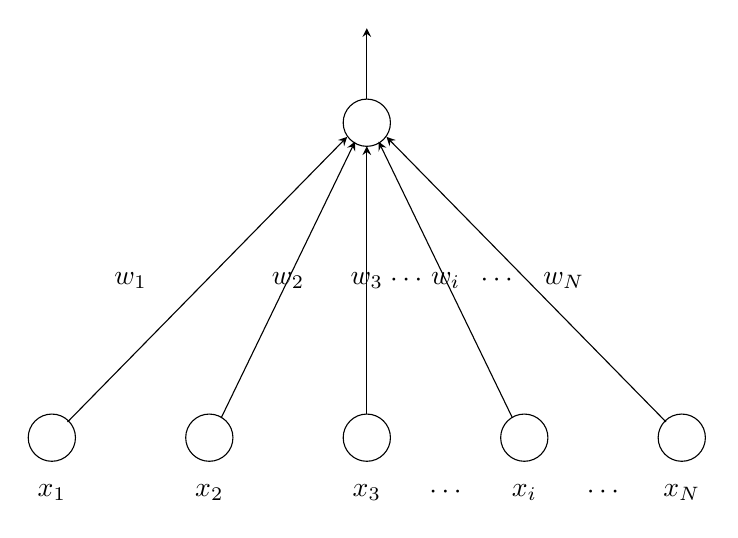
\begin{tikzpicture}[>=stealth]
      \draw(0,0) circle[radius=0.3];
      \draw(-2,0) circle[radius=0.3];
      \draw(2,0) circle[radius=0.3];
      \draw(-4,0) circle[radius=0.3];
      \draw(4,0) circle[radius=0.3];
      \draw(0,4) circle[radius=0.3];
      \draw[->](0,0.3)--(0,3.7);
      \draw[->] (1.85,0.25)--(0.15,3.76);
      \draw[->] (-1.85,0.25)--(-0.15,3.76);
      \draw[->] (3.8,0.2)--(0.25,3.82);
      \draw[->] (-3.8,0.2)--(-0.25,3.82);
      \draw[->] (0,4.3)--(0,5.2);
      \node at(-4,-0.7) {$x_{1}$};
      \node at(-2,-0.7) {$x_{2}$};
      \node at(0,-0.7) {$x_{3}$};
      \node at(1,-0.7) {$\cdots$};
      \node at(2,-0.7) {$x_{i}$};
      \node at(3,-0.7) {$\cdots$};
      \node at(4,-0.7) {$x_{N}$};
      \node at(-3,2) {$w_{1}$};
      \node at(-1,2) {$w_{2}$};
      \node at(0,2) {$w_{3}$};
      \node at(1,2) {$w_{i}$};
      \node at(2.5,2) {$w_{N}$};
      \node at(0.5,2) {$\cdots$};
      \node at(1.65,2) {$\cdots$};
    \end{tikzpicture}
  \end{center}
  $\mbox{\boldmath $x$}^{(k)}=\begin{pmatrix} x_{1}^{(k)}&x_{2}^{(k)}&\cdots&x_{i}^{(k)}&\cdots&x_{N}^{(k)}\end{pmatrix}^{T}$\ :\ 第$k$入力ベクトル\\
  $y^{(k)}$\ :\ 第$k$に対する出力
  \begin{eqnarray*}
    &&y^{(k)}=f\left(\sum_{i=1}^{N}w_{i}x_{i}^{(k)}\right)\\
    &&f(z)=\frac{1}{1+{\rm exp}(-z)}
  \end{eqnarray*}
  カテゴリ$A$であれば1, そうでなければ0とする.\ また\\
  $\mbox{\boldmath $w$}=\begin{pmatrix}w_{1}&w_{2}&\cdots&w_{i}&\cdots&w_{N}\end{pmatrix}$\ :\ 重みベクトル(パーセプトロンのパラメータ)\\
  $t^{(k)}$\ :\ 第$k$入力に対する正解カテゴリ(カテゴリ$A$であれば1そうでなければ0)\\
  $M$\ :\ データの個数\\
  目的関数$H(\mbox{\boldmath $w$})$としたとき目的関数の中身は以下のようになる。
  \begin{eqnarray*}
    H(\mbox{\boldmath $w$})&=&\sum_{j = 1}^{M}\frac{1}{2}\left(y^{(j)}-t^{(j)}\right)^{2}\\
    &=&\sum_{j=1}^{M}\frac{1}{2}\left(f\left(\sum_{i=1}^{N}w_{i}x_{i}{}^{(j)}\right)-t^{(j)}\right)^{2}, f(z)=\frac{1}{1+e^{-z}}\\
  \end{eqnarray*}
  この時最急降下法により、$\mbox{\boldmath $w$}$を求めると次のようになる。\\
  まず更新式は次のようにあらわされる。
  \begin{eqnarray*}
    \mbox{\boldmath $w$}_{n+1}=\mbox{\boldmath $w$}_{n}-\alpha_{n}\frac{\mathrm{\partial} H\left(\mbox{\boldmath $w$}_{n}\right)}{\mathrm{\partial} \mbox{\boldmath $w$}}\\
    \alpha_{n+1}=\beta\alpha_{n}, \alpha_{0}=0.5,\beta=0.98
  \end{eqnarray*}
  ここで、以下の性質が成り立つ
  \begin{eqnarray*}
    H(\mbox{\boldmath $w$})=\sum_{j=1}^{M}\frac{1}{2}\left(y^{(j)}-t^{(j)}\right)^{2},\\
    y^{(j)}=f\left(\sum_{i=1}^{N}w_{i}x_{i}{}^{(j)}\right)\text{の時}\\
    \frac{\mathrm{\partial}}{\mathrm{\partial} w_{i}}H(\mbox{\boldmath $w$})=\sum_{j=1}^{M}\left(y^{(j)}-t^{(j)}\right)y^{(j)}\left(1-y^{(j)}\right)x_{i}{}^{(j)}
  \end{eqnarray*}
  よって、次のことが成り立つ
  \begin{eqnarray*}
    \nabla H(\mbox{\boldmath $w$})
    &=&\frac{\mathrm{\partial}H(\mbox{\boldmath $w$})}{\mathrm{\partial}\mbox{\boldmath $w$}}\\
    &=&[H(\mbox{\boldmath $w$})]% &=&[]
  \end{eqnarray*}
